\chapter{Normalizing Flows}
\label{chapter:probmodel}

\section{Introduction}
The best known and studied probability distributions are rarely expressive
enough for real-world datasets. However, they have properties that make them
amenable to work with, for instance: tractable parameter estimation and closed-form
likelihood functions.

As has been described, one way to obtain more expressive models is to assume the
existence of latent variables, leverage certain factorization structures, and to
use well-known distributions for the individual factors of the product that
constitutes the model's joint distribution. By using these structures and choosing
specific combinations of distributions (namely, conjugate prior-likelihood pairs),
these models are able to stay tractable - normally via bespoke estimation/inference/learning
algorithms.

%Structures are easily encoded by Probabilistic Graphical Models, which are a
%framework to easily express conditional independence assumptions and to specify
%complex probabilistic models.

Another approach to obtaining expressive probabilistic models is to apply
transformations to a simple distribution, and use the Change of Variables
formula to compute probabilities in the transformed space. This is the basis
of Normalizing Flows, an approach proposed by \author{shakir_nf} in \cite{shakir_nf},
and which has since evolved and developed into the basis of multiple SoA techniques
for density estimation [TODO: cite examples here].

\section{Change of Variables}
Given a probability distribution $p(z)$, with probability density function $f_Z(.)$,
and a bijective and continuous function $g$, it's possible to write an expression
for the probability density function $f_Y(.)$ of the random variable $y$ that is
obtained by applying $g$ to samples of $p(z)$:
\begin{align}
    \mbox{if } z &\sim p(z) \\
    \mbox{and } y &= g(z) \\
    \mbox{then } f_Y(y) &= f_Z(g^{-1}(y))\Big|\det\Big(\frac{d}{dy}g^{-1}(y)\Big)\Big|
\end{align}

For this to be useful, some objects have to be easily computable:
\begin{itemize}
    \item $f_Z(z)$ - the starting distribution's probability density function.
        It is assumed that there is a closed-form expression to compute this. In
        practice, this is normally one of the basic distributions (Gaussian,
        Uniform, etc.)
    \item $\det\Big(\frac{d}{dy}g^{-1}(y)\Big)$ - the determinant  of the Jacobian
        matrix of $g^{-1}(.)$ . For most transformations this is not "cheap" to compute.
        As will be shown, the main challenge of Normalizing Flows is to find
        transformations that are expressive and for which 
        the determinants of their Jacobian matrices are "cheap" to compute.
\end{itemize}

\section{Normalizing Flows}
Let us have $L$ transformations $h_\ell$ that fulfill the above two points, and
let $z_\ell$ be the result of applying transformation $h_{\ell-1}$, with the
exception of $z_0$, which is obtained by sampling from $p(z_0)$, the base distribution.
Furthermore, let $g$ be the composition of the $L$ transformations.

Applying the Change of Variables formula:
\begin{align}
    \mbox{if } z_0 &\sim p(z_0) \\
    \mbox{and } y &= h_{L-1} \circ h_{L-2} \circ ... \circ h_0(z_0) \\
    \mbox{then } f_Y(y) &= f_Z(g^{-1}(y))\Big|\det\Big(\frac{d}{dy}g^{-1}(y)\Big)\Big| \\
                        &= f_Z(g^{-1}(y))\prod_{\ell=0}^{L-1}\Big|\det\Big(\frac{d}{dz_{\ell+1}}h_{\ell}^{-1}(z_{\ell+1})\Big)\Big| \\
                        &= f_Z(g^{-1}(y))\prod_{\ell=0}^{L-1}\Big|\det\Big(\frac{d}{dz_{\ell}}h_{\ell}\Big(h_{\ell}^{-1}(z_{\ell+1}\Big)\Big)\Big|^{-1} \label{eq:nflowderivation}
\end{align}

Replacing $h_{\ell}^{-1}(z_{\ell+1}) = z_\ell$ in \ref{eq:nflowderivation}:

\begin{align}
         f_Y(y) &= f_Z(g^{-1}(y))\prod_{\ell=0}^{L-1}\Big|\det\Big(\frac{d}{dz_{\ell}}h_{\ell}\Big(z_\ell)\Big)\Big)\Big|^{-1} \\
    \log f_Y(y) &= \log f_Z(g^{-1}(y)) - \sum_{\ell=0}^{L-1} \log \Big|\det\Big(\frac{d}{dz_{\ell}}h_{\ell}(z_\ell)\Big) \Big| \label{eq:nflowsfinal}
\end{align}

Depending on the task, one might prefer to replace the second term in \ref{eq:nflowsfinal}
with a sum of log-abs-determinants of the Jacobians of the inverse transformations.
This switch would imply replacing the minus sign before the sum with a plus sign:
\begin{align}
    \log f_Y(y) &= \log f_Z(g^{-1}(y)) + \sum_{\ell=0}^{L-1} \log \Big|\det\Big(\frac{d}{dz_{\ell+1}}h_{\ell}^{-1}(z_{\ell+1})\Big) \Big|
\end{align}

With this expression, gradient-based MLE becomes feasible. Moreover, sampling
from the resulting distribution is simply achieved by sampling from the base
distribution and applying the chain of transformations. Because of this, Normalizing
Flows lend themselves to be used as flexible variational posteriors, in Variational
Inference settings.

\section{Examples of transformations}
\subsection{Affine Transformation}
The simplest transform that can be applied is an Affine transformation.
This transformation can stretch, shrink and rotate space. It is simply the 
multiplication by a matrix $A$ and summation of a bias vector $b$:
\begin{align}
    z &\sim p(z) \\
    y &= Az + b
\end{align}

The Jacobian of this transformation is simply the determinant of the matrix $A$.

However, in general, computing the determinant of a $N \times N$ matrix has a
complexity of $\mathcal{O}(N^3)$. For that reason, it is common to use matrices
with a certain structure that makes their determinants easier to compute. For
instance, if $A$ is triangular, its determinant is simply the product of its
diagonal's elements. The downside of using matrices that are constrained to
a certain structure is that they correspond to less flexible transformations.

It is possible, however, to design Affine transformations whose Jacobians are
of $\mathcal{O}(N)$ complexity and that are more expressive than simple
triangular matrices. In \cite{Glow}, one such transformation is proposed. It
constrains the matrix $A$ to be decomposable as $A = PL\big(U + diag(\mathbf{s})\big)$,
where $diag(\mathbf{s})$ is a diagonal matrix whose diagonal's elements are
the values of vector $\mathbf{s}$. The following additional constrains are in place:
\begin{itemize}
    \item $P$ is a permutation matrix
    \item $L$ is a lower triangular matrix, with ones on its diagonal
    \item $U$ is an upper triangular matrix, with zeros on its diagonal
\end{itemize}

Given these constraints, the determinant of the matrix $A$ is simply the product
of the elements of $\mathbf{s}$.

\begin{figure}[!htb]
  \begin{subfigmatrix}{2}
    \subfigure[]{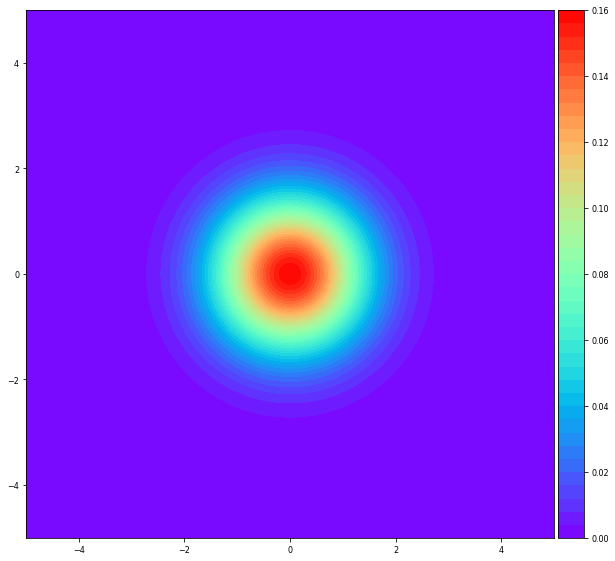
\includegraphics[width=0.49\linewidth]{figures/base_distribution.png}}
    \subfigure[]{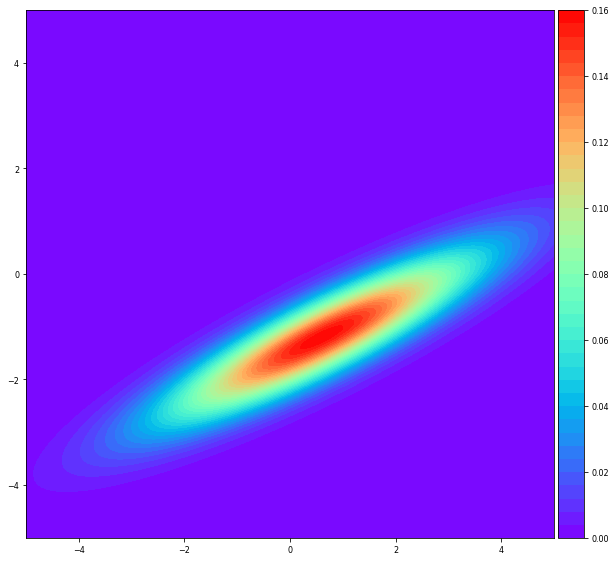
\includegraphics[width=0.49\linewidth]{figures/affine_transform.png}}
  \end{subfigmatrix}
    \caption{(a) Density of a Gaussian distribution with $\mu = [0, 0]$ and $\Sigma = I$
    (b) Density of the distribution that results from applying some affine transformation to
    the Gaussian distribution in (a)
    }
  \label{fig:affine}
\end{figure}

\subsection{PReLU Transformation}
Intuitively, introducing non-linearity endows Normalizing Flows with more flexibility to 
represent complex distributions. This can be done in similar fashion to the
activation functions of neural networks. One example of that, is the Parameterized
Rectified Linear Unit transformation. It is defined in the following manner, for
a $d$-dimensional input:
\begin{align}
f_i(z_i) =
    \begin{cases}
        z_i,              & \text{if } z_i\geq 0\\
        \alpha z_i,       & \text{otherwise}
    \end{cases} \\
f(\mathbf{z}) = [f_0(z_0), f_1(\mathbf{z_1}), ..., f_d(z_d)]
\end{align}

Note that in order for the transformation to be invertible, it is necessary
that $\alpha > 0$.

Let us define an auxiliary function $j(.)$ s.t.:
\begin{align}
j(z_i) =
    \begin{cases}
       1 ,              & \text{if } z_i \geq 0\\
       \alpha ,       & \text{otherwise}
    \end{cases}
\end{align}

It's trivial to see that the jacobian of the transformation is a diagonal
matrix, whose diagonal elements are $j(z_i)$:
\begin{align}
  A =
  \begin{bmatrix}
      j(z_0) & & & \\
      & j(\mathbf{z_1}) & & \\
      & & \ddots & \\
      & & & j(z_d)
  \end{bmatrix}
\end{align}

With that, it is easy to arrive at the log-abs-determinant of this transformantion's
jacobian, which is given by $\sum_{i=0}^d \log \Big| j(z_i) \Big|$

\begin{figure}[!htb]
  \begin{subfigmatrix}{2}
    \subfigure[]{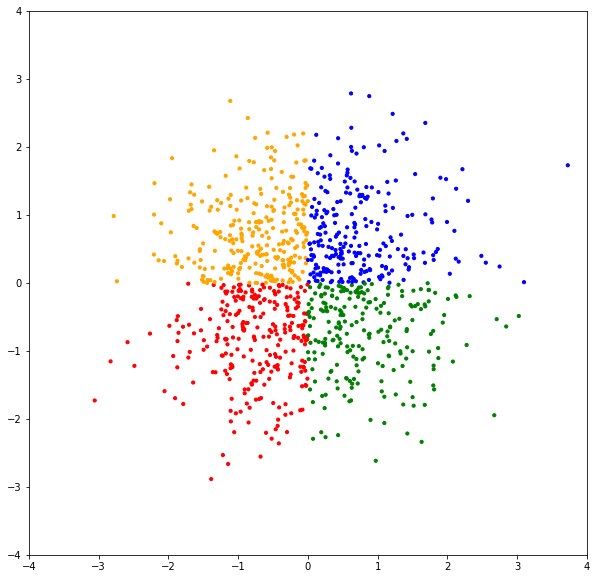
\includegraphics[width=0.49\linewidth]{figures/gaussian_in_quadrants.png}}
    \subfigure[]{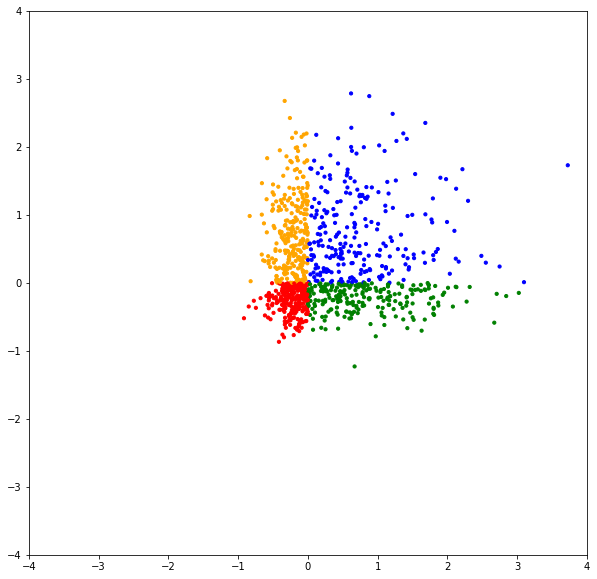
\includegraphics[width=0.49\linewidth]{figures/prelu_in_quadrants.png}}
  \end{subfigmatrix}
    \caption{(a) Samples from of a Gaussian distribution with $\mu = [0, 0]$ and $\Sigma = I$.
    The samples are colored according to the quadrant they belong to. (b) Samples from the
    distribuion in a) transformed by a PReLU transformation.}
  \label{fig:prelu}
\end{figure}

\begin{figure}[!htb]
  \begin{subfigmatrix}{3}
    \subfigure[]{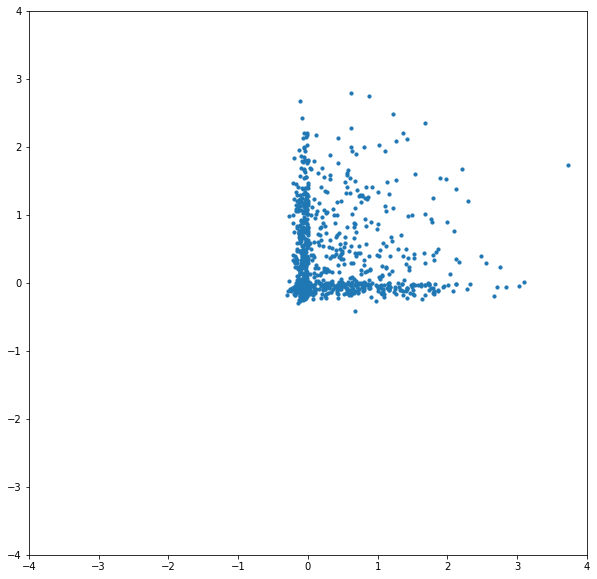
\includegraphics[width=0.31\linewidth]{figures/prelu_0_1.png}}
    \subfigure[]{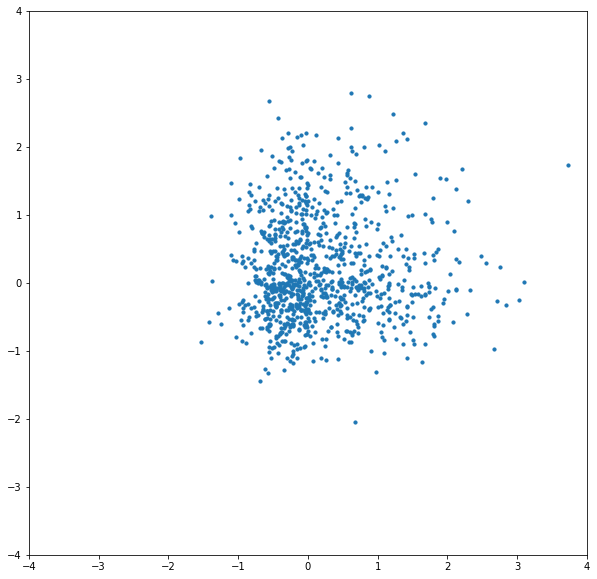
\includegraphics[width=0.31\linewidth]{figures/prelu_0_5.png}}
    \subfigure[]{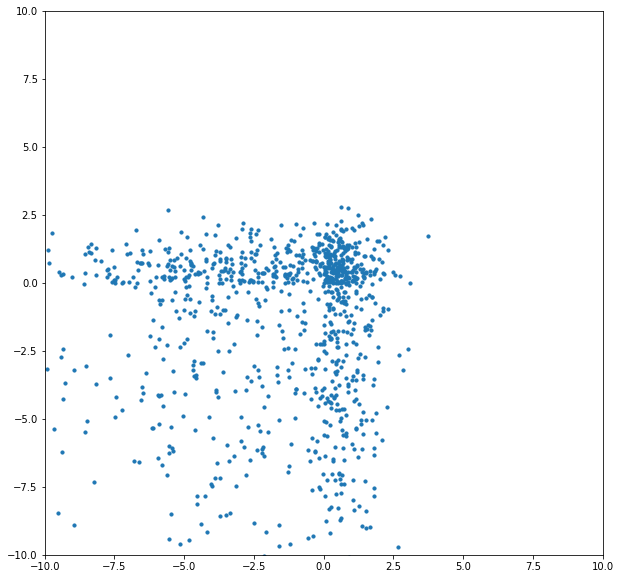
\includegraphics[width=0.31\linewidth]{figures/prelu_5.png}}
  \end{subfigmatrix}
    \caption{Samples from a Gaussian with $\mu = [0, 0]$ and $\Sigma = I$, transformed
    by PReLU transformations with different $\alpha$ parameters. (a) $\alpha = 0.1$
    (b) $\alpha = 0.5$ (c) $\alpha = 5$}
  \label{fig:prelu}
\end{figure}

\subsection{Batch-Norm Transformation}
In \cite{realnvp}, the authors propose a Batch-Norm transformation, similar to
the Batch-Norm layer normally used in neural networks. This transform simply
applies a rescaling, given as a function the batch mean $\tilde\mu$ and variance
${\tilde\sigma}^2$:
\begin{align}
    f(z) = \frac{z - \tilde\mu}{\sqrt{{\tilde\sigma}^2 + \epsilon}},
\end{align} where $\epsilon \ll 1$ is a term used to ensure that there never is
a division by zero.

This transformation's Jacobian is trivial: 
\begin{align}
    \prod \frac{1}{\sqrt{{\tilde\sigma}_i^2 + \epsilon}}
\end{align}

\subsection{Affine Coupling Transformation}
As mentioned previously, one of the active research challenges within the
Normalizing Flows framework is the search and design of transformations that
are expressive and whose Jacobians are not computationally heavy. One brilliant
example of such transformation was proposed by \cite{author:real-nvp} in
\cite{real-nvp}, and is called Affine Coupling Layer.

This transformation is characterized by two \textbf{arbitrary} functions $s(.)$ and
$t(.)$, as well as a mask that splits an input $\mathbf{z}$ of dimension $D$ into
two parts, $\mathbf{z_1}$ and $\mathbf{z_2}$. In practice, $s(.)$ and $t(.)$ are
neural networks, whose parameters will be optimized so as to make the transformation
approximate the desired output distribution. The outputs of $s(.)$ and $t(.)$
need to have the same dimension as $z_1$. This should be taken into account when
designing the mask and the functions $s(.)$ and $t(.)$.

It is defined as:

\begin{align}
    \mathbf{x_1} &= \mathbf{z_1} \odot \exp\big(s(\mathbf{z_2})\big) + t(\mathbf{z_2}) \\
    \mathbf{x_2} &= \mathbf{z_2}
\end{align}

To see why this transformation is suitable to being used within the framework
of Normalizing Flows, let us derive its Jacobian.
\begin{itemize}
    \item $\frac{\partial \mathbf{x_2}}{\partial \mathbf{z_2}} = \mathbb{I}$ is trivial, because $\mathbf{x_2} = \mathbf{z_2}$.
    \item $\frac{\partial \mathbf{x_2}}{\partial \mathbf{z_1}}$ is a matrix of zeros, and it is also
        trivial, because $\mathbf{x_2}$ does not depend on $\mathbf{z_1}$.
    \item $\frac{\partial \mathbf{x_1}}{\partial \mathbf{z_1}}$ is a diagonal matrix,
        whose diagonal is simply given by $\exp\big(s(\mathbf{z_2})\big)$, since those values are
        constant w.r.t $\mathbf{z_1}$ and they are multiplying each element of $\mathbf{z_1}$.
    \item $\frac{\partial \mathbf{x_1}}{\partial \mathbf{z_2}} = 1$ is not needed for our purposes,
        as will become clear ahead.
\end{itemize}

Writing the above in matrix form:
%\[
%\begin{bmatrix}
%  \mbox{\huge$\frac{\partial \mathbf{x_1}}{\partial \mathbf{z_1}}$} & \mbox{\huge$\frac{\partial \mathbf{x_1}}{\partial \mathbf{z_2}}$} \\
%  \mbox{\huge$\frac{\partial \mathbf{x_2}}{\partial \mathbf{z_1}}$} & \mbox{\huge$\frac{\partial \mathbf{x_2}}{\partial \mathbf{z_2}}$} \\
%\end{bmatrix}
%\]


\begin{align}
    J_{f(z)} &=
        \begin{tikzpicture}[decoration=brace, baseline=-\the\dimexpr\fontdimen22\textfont2\relax ]
            \matrix (m) [matrix of math nodes,left delimiter=[,right delimiter={]}, ampersand replacement=\&] {
                \mbox{\Large$\frac{\partial \mathbf{x_1}}{\partial \mathbf{z_1}}$} \& \mbox{\Large$\frac{\partial \mathbf{x_1}}{\partial \mathbf{z_2}}$} \\
                \mbox{\Large$\frac{\partial \mathbf{x_2}}{\partial \mathbf{z_1}}$} \& \mbox{\Large$\frac{\partial \mathbf{x_2}}{\partial \mathbf{z_2}}$} \\
            };
%            \draw[decorate,transform canvas={xshift=-1.5em},thick] ($ (m-1-1.south west) +(0,3pt) $)
%                -- node[left=2pt] {$\frac{\partial \mathbf{x_1}}{\partial (.)}$} ($ (m-1-1.north west) -(0,3pt) $);
%            \draw[decorate,transform canvas={xshift=-1.5em},thick] ($ (m-2-1.south west) +(0,3pt) $)
%                -- node[left=2pt] {$\frac{\partial \mathbf{x_2}}{\partial (.)}$} ($ (m-2-1.north west) -(0,3pt) $);
%            \draw[decorate,transform canvas={yshift=0.5em},thick] ($ (m-1-1.north west) +(2pt,0) $)
%                -- node[above=2pt] {$\frac{\partial (.)}{\partial \mathbf{z_1}}$} ($ (m-1-1.north east) -(2pt,0) $);
%            \draw[decorate,transform canvas={yshift=0.5em},thick] ($ (m-1-2.north west) +(2pt,0) $)
%                -- node[above=2pt] {$\frac{\partial (.)}{\partial \mathbf{z_2}}$} ($ (m-1-2.north east) +(2pt,0) $);
        \end{tikzpicture} \\
    &=
        \begin{tikzpicture}[decoration=brace, baseline=-\the\dimexpr\fontdimen22\textfont2\relax ]
            \matrix (m) [matrix of math nodes,left delimiter=[,right delimiter={]}, ampersand replacement=\&] {
                \exp\big(s(\mathbf{z_2})\big) \& \mbox{\Large$\frac{\partial \mathbf{x_1}}{\partial \mathbf{z_2}}$} \\
                \mbox{\Large$\mathbf{0}$} \& \mbox{\Large$\mathbb{I}$} \\
            };
        \end{tikzpicture}
\end{align}

The Jacobian matrix is triangular. Its determinant - the only thing we need,
in fact - is therefore easy to compute: it is simply the product of the diagonal.
Moreover, part of the diagonal is simply composed of ones. The determinant, and
the log-abs-determinant become:

\begin{align}
    det\big(J_{f(z)}\big) &= \prod_i \exp\big(s(\mathbf{z_2}^{(i)})\big) \\
    \log \Big|det\big(J_{f(z)}\big)\Big| &= \sum_i s(\mathbf{z_2}^{(i)}),
\end{align}

where $\mathbf{z_2^{(i)}}$ is the $i$-th element of $\mathbf{z_2}$.

Since a single Affine Coupling Layer doesn't transform all of the elements in
$\mathbf{z}$, in practice several layers are stacked on top of each other, and
each layer's mask is changed so as to make all dimensions affect each other.
This can be done for instance with a checkerboard pattern, which alternates
for each layer. In the case of image inputs, the masks can operate at the channel
level.

\section{Fitting Normalizing Flows}

Generally speaking, Normalizing Flows can be used in one of two scenarios:
(direct) density estimation, where the goal is to optimize the NF's parameters
so as to make the model approximate the distribution of some observed data;
in a variational inference scenario, as way to have a flexible variational
posterior (i.e. $q(z)$ in the terminology used in the previous chapter). The
second scenario is out of the scope of this work.

The task of density estimation with Normalizing Flows reduces to finding the
optimal parameters of a parametric model. As mentioned in \ref{section:map-mle},
there are two ways to go about estimating the parameters of a parametric model,
given data: MLE and MAP. In the case of Normalizing Flows, MLE is the usual
approach\footnote{In theory it is possible to place a prior on the NF's parameters
and do MAP estimation. To accomplish this, similar strategies to those used in
Bayesian Neural Networks would have to be used.}. To fit a Normalizing Flow via
MLE, a gradient based optimizer is used to minimize
$\hat{\mathcal{L}}(\theta) = - \mathbb{E}[\log p(x|\theta)]$
